\section{Equivalência de Recursos}
\label{sec:equivalenciaRecursos}

Entende-se por equivalência tudo aquilo que tem o mesmo valor.

\begin{quote}
	Lucas estava brincando com seu carrinho, quando uma das rodinhas se quebrou. Entristecido, ele procurou por seu pai, que, ao ver a aflição de seu filho, resolveu ajudar. Recolheu uma garrafa PET que estava por perto, desenroscou sua tampinha e a colocou no lugar deixado pela rodinha estragada. Tamanha foi a felicidade de Lucas ao poder voltar a brincar com o seu carrinho.
\end{quote}

A história acima, apesar de simples, contém informações que podem ser úteis. Observe que os objetos envolvidos, ou seja, a rodinha e a tampinha, diferem na maioria das suas características: material, valor, peso, cor, etc. Apesar de tudo, pelo menos uma das características é igual: ambas possuem formatos cilíndricos. Foi essa única semelhança que permitiu o conserto do carrinho e garantiu a felicidade de Lucas! Ou seja, no contexto apresentado, a rodinha e a tampinha puderam ser trocadas sem perda de valor.

É exatamente esse o sentido ao se afirmar que dois recursos são equivalentes. Um não precisa ser igual ao outro, mas apenas possuir uma característica que, em determinado momento, possibilite a intercambialidade. Seria possível, por exemplo, utilizar um \emph{joystick} como um dispositivo apontador e, a qualquer momento, substitui-lo por um \emph{laser pointer} de forma que os serviços necessários continuassem sendo providos. Repare que tais dispositivos, assim como a rodinha e a tampinha, são bastante diferentes em diversas de suas características, mas ainda assim são capazes de fornecer serviços iguais, como mover uma seta pela tela.

\subsection{Cálculo de Equivalência}

Para garantir que determinado recurso seja equivalente a outro, deve-se considerar o conjunto de serviços presentes em cada recurso envolvido, bem como as suas relações. Admita que a notação $A \implies B$ denote que um recurso A é equivalente a um recurso B e considere as afirmações abaixo:

\begin{enumerate}
	\item $R1 \implies R2$;
	\item $R2 \implies R3$.
\end{enumerate}

A partir delas e, com base na figura~\ref{fig:calculoDeEquivalencia}, tome as seguintes regras:

\begin{figure}[ht]
	\center
	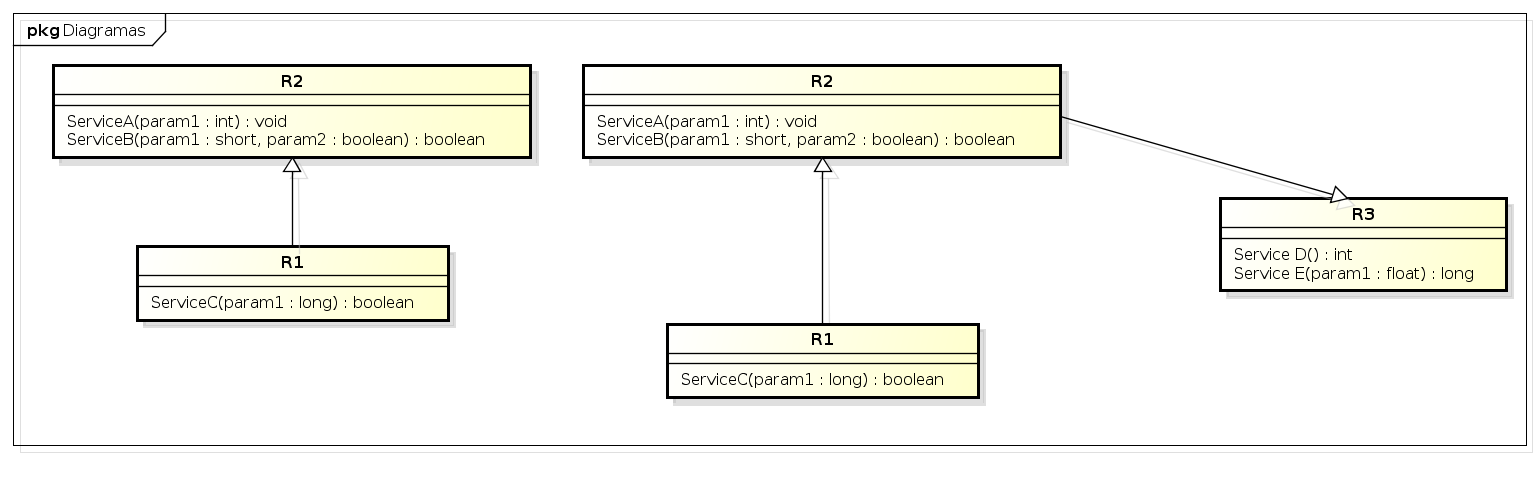
\includegraphics[scale=0.39]{imagens/calculoDeEquivalencia}
	\caption{Cálculo de equivalência: exemplo de recursos equivalentes.}
	\label{fig:calculoDeEquivalencia}
\end{figure}

\begin{itemize}
	\item Consistência de serviços

		Os serviços providos por R2 devem existir em R1. Observe que tal obrigação não impede que R1 contenha outros serviços desconhecidos por R2. Caso todos os serviços em R1 sejam iguais aos serviços em R2, tais recursos são iguais e não equivalentes.
	\item Consistência de interface

		As interfaces dos serviços providos por R2 que também estão em R1 devem ser idênticas. Isso implica em dizer que os nomes dos serviços devem ser iguais, bem como os seus parâmetros.

		Parte-se do princípio que não existirá interesse em camuflar um serviço malicioso ao expor uma interface compatível com a equivalência.
	\item Refência circular

		Não é permitida.
\end{itemize}

\begin{comment}
Para que um recurso R1 seja equivalente a um recurso R2, os serviços de R2 deverão estar presentes no conjunto de serviços de R1, mas R1 poderá ter outros serviços que não estão presentes em R2. Seja S(X), o conjunto de serviços do recurso X, então teríamos que $S(R1) \cap S(R2) = S(R2)$. 

\begin{figure}[ht]
	\center
	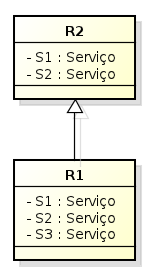
\includegraphics[scale=0.6]{imagens/equivalenciaDeRecursos}
	\caption{Exemplo de recursos equivalentes.}
	\label{fig:equivalenciaDeRecursos}
\end{figure}

Suponha uma situação em que $A \implies B$, $B \implies C$ e $C \implies A$, logo teríamos que $A \implies C$, o que seria uma relação circular, o que não faz sentido, pois concluiríamos que todos os recursos são iguais e não equivalentes. Devemos, portanto, garantir que não ocorra essa equivalência circular. Caso algum dispositivo queira registrar um novo \emph{driver} que cause essa inconsistência, devemos impedir que essa inconsistência possa ocorrer, ou então alertar o novo driver da ocorrência deste problema e não realizar seu registro.

\subsubsection{Consistência de Interface}

	A figura~\ref{fig:consistenciaInterface} mostra que o recurso R1 é equivalente ao recurso R3, mas embora possua um serviço de mesmo nome que o recurso R2,  seus parâmetros são diferentes, logo, não pode ser um mesmo serviço e os recursos não serão equivalentes..
	
	Para garantir que os recursos são equivalentes, devemos realizar três validações nas interfaces de cada serviço dos recursos:
	\begin{enumerate}
		\item Recurso:
			
			Os serviços devem pertencer ao mesmo recurso cujas classes padrões foram definidas anteriormente.
		
		\item Identificador do Serviço:

			Os serviços devem possuir os mesmos identificadores.

		\item Parâmetros:

			Os serviços devem possuir os mesmos parâmetros.
	\end{enumerate}

	Parte-se do princípio que não existirá interesse em camuflar um serviço malicioso ao expor uma interface compatível com a equivalência.

\begin{figure}[ht]
	\center
	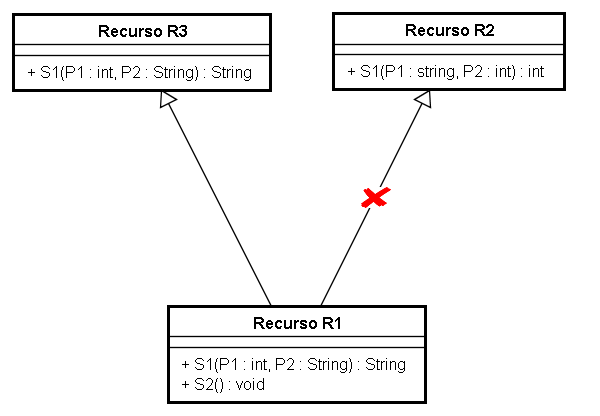
\includegraphics[scale=0.8]{imagens/consistenciaInterface}
	\caption{Exemplo de inconsistência de interface.}
	\label{fig:consistenciaInterface}
\end{figure}
\end{comment}

\begin{comment}
----------------------------------------- REVER ----------------------------------------- \\
Desta forma, faz-se necessária uma maneira de classificar tais recursos imersos nos mais variados dispositivos presentes no \emph{smart space} e regidos pelo \emph{middleware}. Essa classificação facilitará o desenvolvimento de novos \emph{drivers} para futuras aplicações, pois tornará possivel a definição de interfaces pré-estabelecidas que representem classes de recursos. Outra vantagem decorrente é a possibilidade de seleção de recursos equivalentes, caso o provedor originalmente selecionado esteja indisponível. \\
----------------------------------------- REVER -----------------------------------------

COLOQUEI NO COMEÇO DA PROPOSTA
\end{comment}

\subsection{Árvore de Recursos}

Cada uma dessas classes servirá de raiz para uma árvore de recursos, ou seja, existirão diversas árvores, cada qual com outras classes agrupadas por funcionalidades. Para tornar tal estrutura mais clara, considere a figura~\ref{fig:arvoreDeRecursos}. Observe a hierarquia formada a partir da classe padrão \emph{Pointer}. Ela é responsável por agrupar todas as classes de recursos capazes de prover serviços relacionados aos apontadores existentes, por exemplo, \emph{click} e \emph{scroll}. O mesmo acontece com as demais classes padrões. A estrutura em árvore é importante pois permite uma melhor organização lógica das classes relacionadas, além de permitir uma fácil navegabilidade entre elas.

\begin{figure}[ht]
	\center
	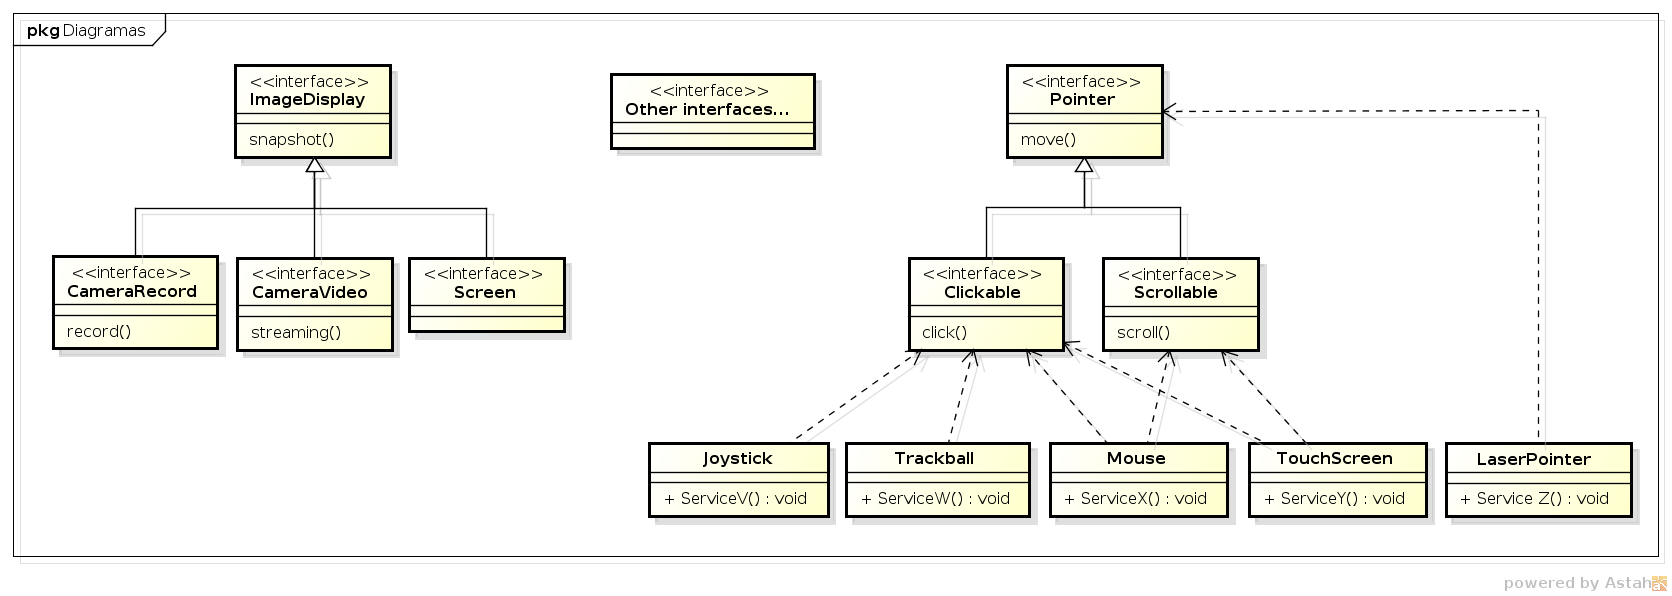
\includegraphics[scale=0.35]{imagens/hierarquiaDeRecursos}
	\caption{Exemplo da estrutura de árvores de recursos.}
	\label{fig:arvoreDeRecursos}
\end{figure}

Uma vez que tal estrutura esteja construída, torna-se simples descobrir todos os recursos equivalentes a quaisquer classes presentes na árvore. Para tal, basta tomar a subárvore cuja raiz é o elemento ao qual deseja-se obter seus equivalentes. Observe a figura~\ref{fig:tutorialDeEquivalencia} e imagine que seja necessário oferecer todos os recursos equivalentes à classe \emph{Clickable}. Ao se colocar tal classe como raiz de sua subárvore, torna-se fácil perceber que as classes \emph{Joystick}, \emph{Trackball}, \emph{Mouse} e \emph{TouchScreen} são suas equivalentes.

\begin{figure}[ht]
	\center
	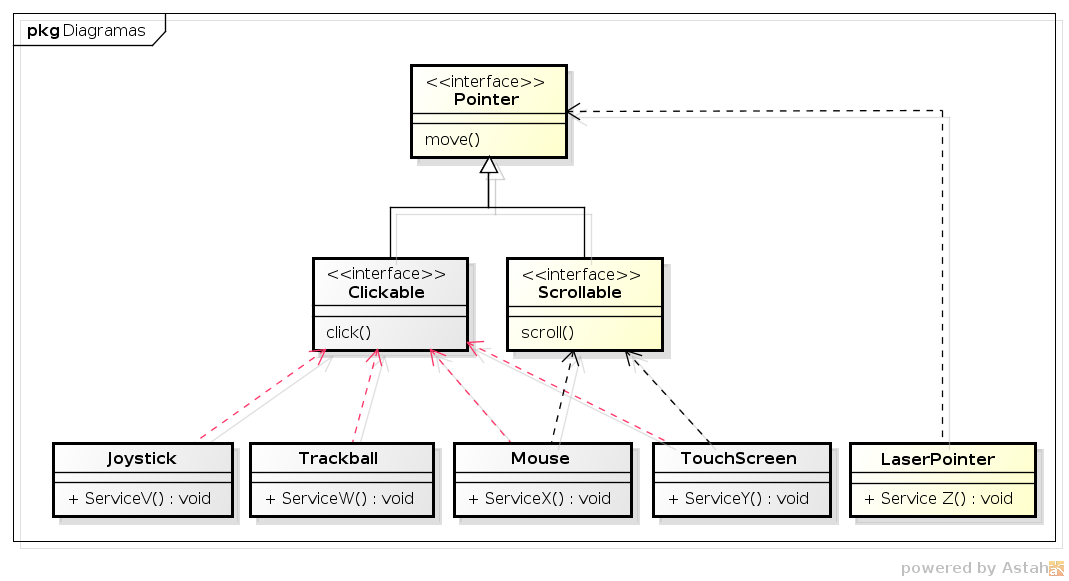
\includegraphics[scale=0.55]{imagens/tutorialDeEquivalencia}
	\caption{Exemplo de como se encontrar recursos equivalentes.}
	\label{fig:tutorialDeEquivalencia}
\end{figure}